\documentclass{article}
%\usepackage[margin=1in]{geometry}
\usepackage{graphicx} % Required for inserting images
\usepackage{hyperref}
\usepackage{amsmath}
\usepackage{titling}
\usepackage{enumitem}
\usepackage{makecell}
\usepackage{minted}
\usepackage{url}
\usepackage{tabularx}
\usepackage{graphicx}
\renewcommand\maketitlehooka{\null\mbox{}\vfill}
\renewcommand\maketitlehookd{\vfill\null}

\begin{document}
\centering

\title{\Huge Intro Deep Learning Homework 1}

\author{ \huge
Jaskin Kabir \\
\Large Student Id: 801186717 \\
\Large \href{https://github.com/jaskinkabir/Intro_Deep_Learning/tree/master/HM1}{GitHub:}\\\url{https://github.com/jaskinkabir/Intro_Deep_Learning/tree/master/HM1}
}

\date{January 2025}

\begin{titlingpage}
\maketitle
\end{titlingpage}

\section{Problem 1: Character Prediction Small Dataset}

\begin{enumerate}[label=1\alph*. ]
    \item \textit{Training Curves}
    \begin{figure}[htb]
        \setkeys{Gin}{width=\linewidth}
        \setlength\tabcolsep{2pt}
        \begin{tabularx}{\textwidth}{XXX}
          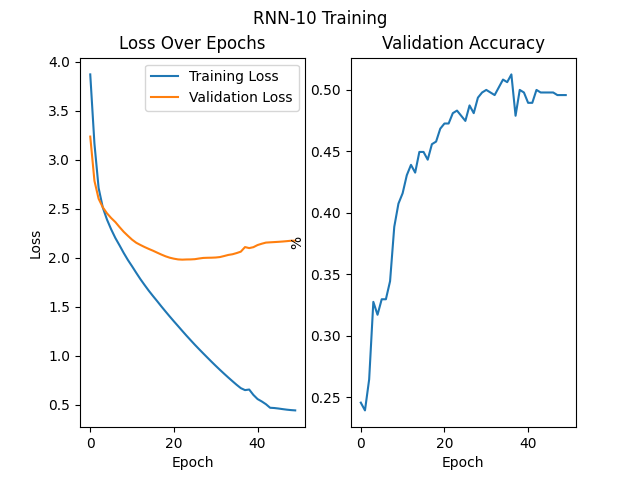
\includegraphics{images_p1/RNN_10_training_new.png} &
          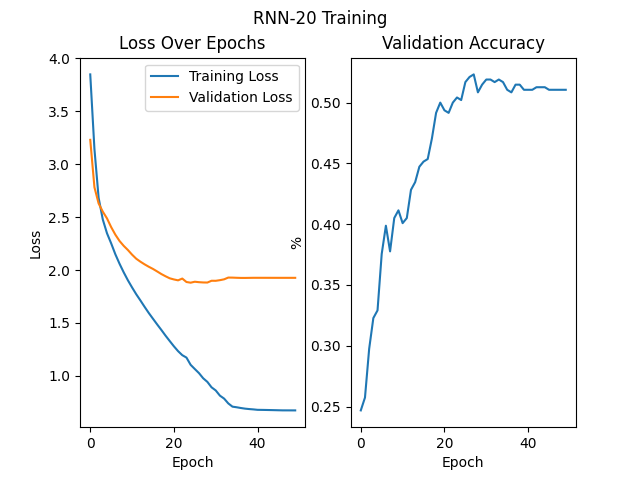
\includegraphics{images_p1/RNN_20_training_new.png} &
          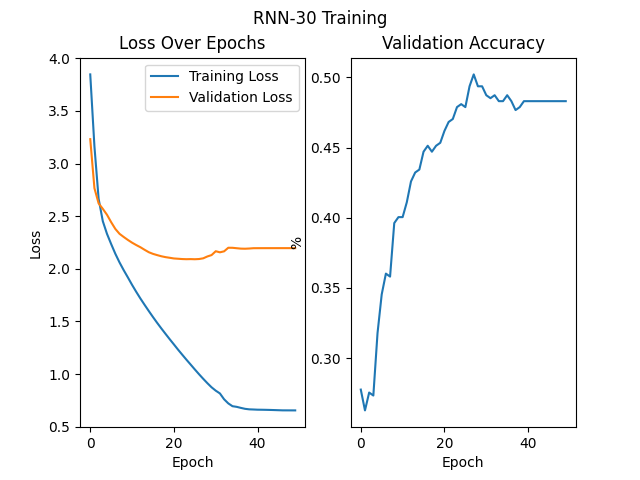
\includegraphics{images_p1/RNN_30_training_new.png}   \\
          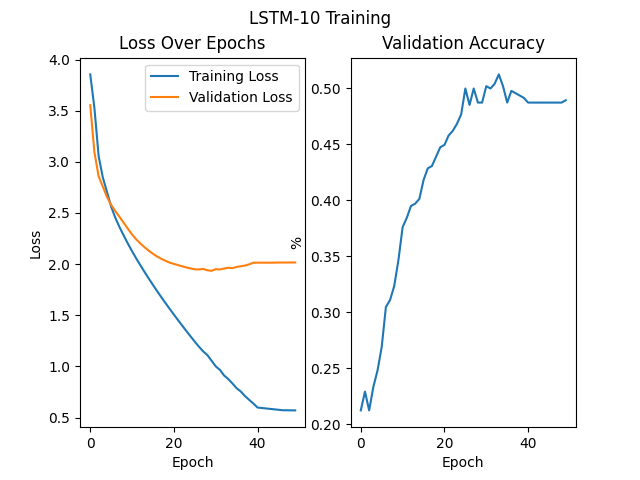
\includegraphics{images_p1/LSTM_10_training_new.png} &
          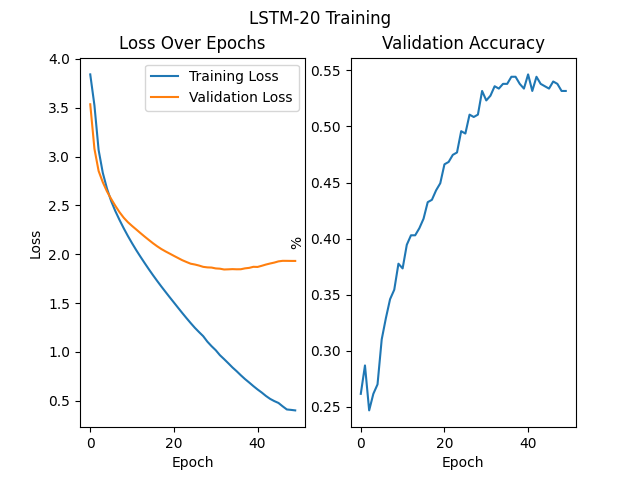
\includegraphics{images_p1/LSTM_20_training_new.png} &
          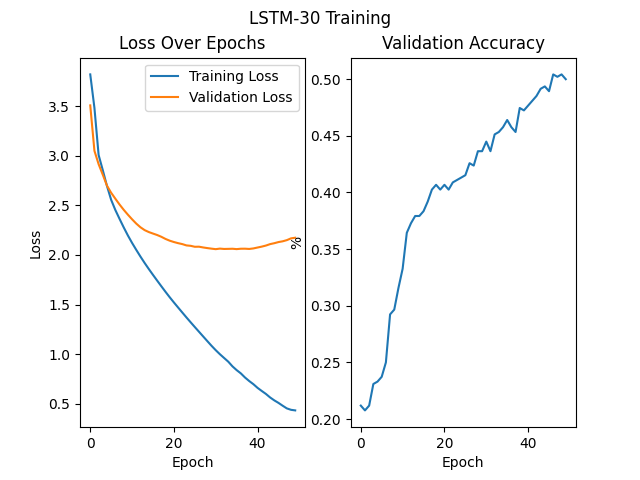
\includegraphics{images_p1/LSTM_30_training_new.png}   \\
          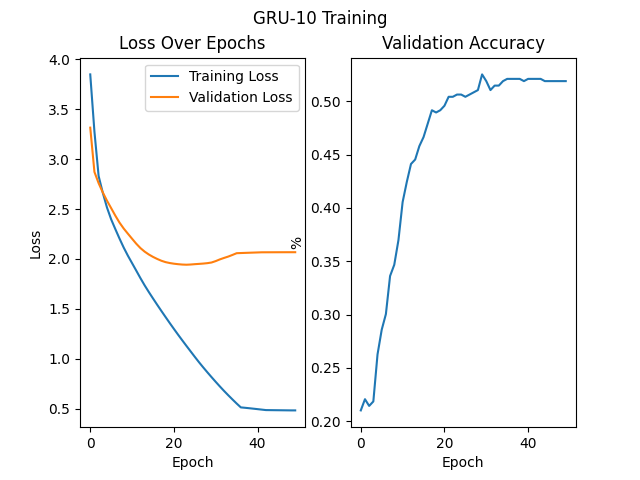
\includegraphics{images_p1/GRU_10_training_new.png} &
          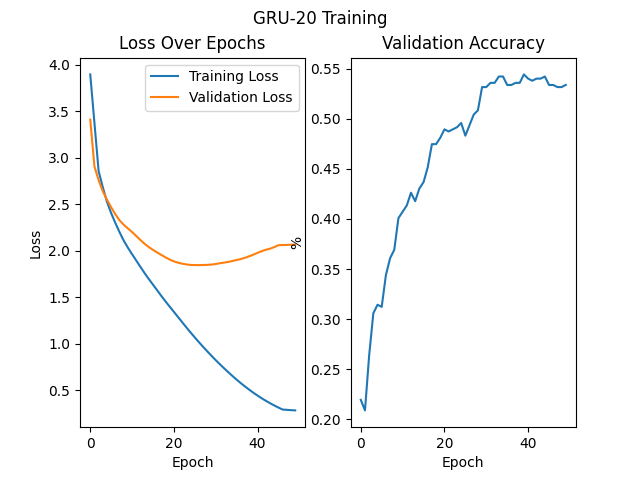
\includegraphics{images_p1/GRU_20_training_new.png} &
          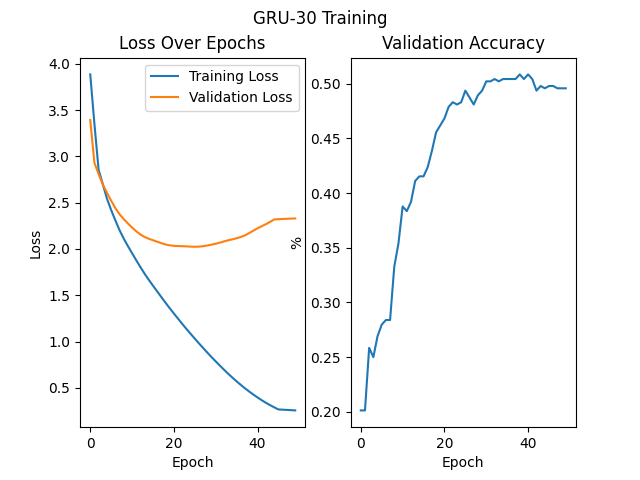
\includegraphics{images_p1/GRU_30_training_new.png}
        \end{tabularx}
        \caption{Problem 1 Training Curves}
        \label{fig:p1}
      \end{figure}
    \item \textit{Results Comparison}
    \begin{table}[h]
        \centering
        \renewcommand{\arraystretch}{1.5}
        \begin{tabular}{|>{\centering\arraybackslash}m{3cm}|>{\centering\arraybackslash}m{3cm}|>{\centering\arraybackslash}m{3cm}|>{\centering\arraybackslash}m{3cm}|>{\centering\arraybackslash}m{3cm}|}
        %\begin{tabular}{|l|r|r|r|r|}
            \hline
            \textbf{Model} & \textbf{Parameter Count} & \textbf{Training Time (s)} & \textbf{Overfit (\%)} & \textbf{Accuracy (\%)} \\
            \hline
            \textbf{RNN-10}  & 44846  & 1.93  & 389.68  & 49.58 \\
            \textbf{RNN-20}  & 44846  & 3.65  & 185.97  & 51.05 \\
            \textbf{RNN-30}  & 44846  & 5.24  & 235.41  & 48.31 \\
            \hline
            \textbf{LSTM-10} & 143918 & 5.79  & 253.80  & 48.95 \\
            \textbf{LSTM-20} & 143918 & 11.21 & 381.00  & 53.16 \\
            \textbf{LSTM-30} & 143918 & 18.23 & 399.18  & 50.00 \\
            \hline
            \textbf{GRU-10}  & 110894 & 5.30  & 329.01  & 51.89 \\
            \textbf{GRU-20}  & 110894 & 9.88  & 633.11  & 53.38 \\
            \textbf{GRU-30}  & 110894 & 15.41 & 460.00  & 50.85 \\
            \hline
        \end{tabular}
        \caption{Problem 1 Data Comparison}
        \label{tab:p1}
    \end{table}
    \item \textit{Discussion} 
    
    The parameter count of the LSTM network was more than
    triple that of the basic RNN network, and the GRU was
    almost halfway between the two. In terms of training
    time, the RNN was the quickest to train, followed by the
    GRU and then the LSTM. This is to be expected, as the
    LSTM adds significant complexity to the base RNN
    architecture, and the GRU reduces that complexity. This
    complexity comes from the number of gates in each
    architecture. The RNN-20 model had the lowest overfit,
    while the LSTM-30 model had the highest. The GRU-20
    model had the highest accuracy, while the RNN-30 model
    had the lowest.
    


\end{enumerate}


\end{document}